\section{Problem and Significance}
The biggest problem of AI is no longer its perceived utility, as this has mostly been solved by its recent successes, but its capacity to \textit{elicit the trust of users}.
The creators of an automated system should be able to make it be trusted in a manner proportional to the criticality of its application. \citep{gilpin2018explaining}, \citep{abdul2018trends}
The potential lack of trust felt by users stems from the difficulty in \textit{verifying the system's outputs}; if no rationale can be inferred for why a given ML model made a certain decision, there is also no way to understand if these outputs conform to our moral norms\footnote{See \citet{gilpin2018explaining} and \citet{abdul2018trends} for a discussion on trust in AI.}.
As discussed in Section \ref{sec:importance-of-explainability}, no explicit justification for the link between the explainability and the \textit{trustability} of a model has been found in the reviewed literature; nonetheless, it seems quite natural to infer that a person would not trust decisions made on an unknown rationale. 
Unfortunately, the \textit{explainability} and performance of machine learning models are usually inversely proportional, as is shown in Figure \ref{fig:darpa-comparison-methods}.

There are many examples of modern methods - such as boosted trees, random forests, bagged trees, kernelized-SVMs - that show the tendency outlined in Figure \ref{fig:darpa-comparison-methods}, but it is best exemplified by \textit{deep neural networks} (DNNs). 
Deep neural networks are machine learning models constructed by stacking many layers of artificial neurons; these systems currently offer state of the art performance on a variety of tasks but are among the least interpretable systems due to the fact that they represent information in an \textit{implicit} (non-symbolic) and \textit{distributed} manner.  
Some older models, like decision trees or rule-based methods, are inherently more interpretable due to their simplicity and the fact that they can explicitly demonstrate their reasoning steps, but are less accurate and flexible than more modern techniques. \citep{Biran2017} (as exemplified in Figure \ref{fig:darpa-comparison-methods})

\begin{figure}[htbp]
\centerline{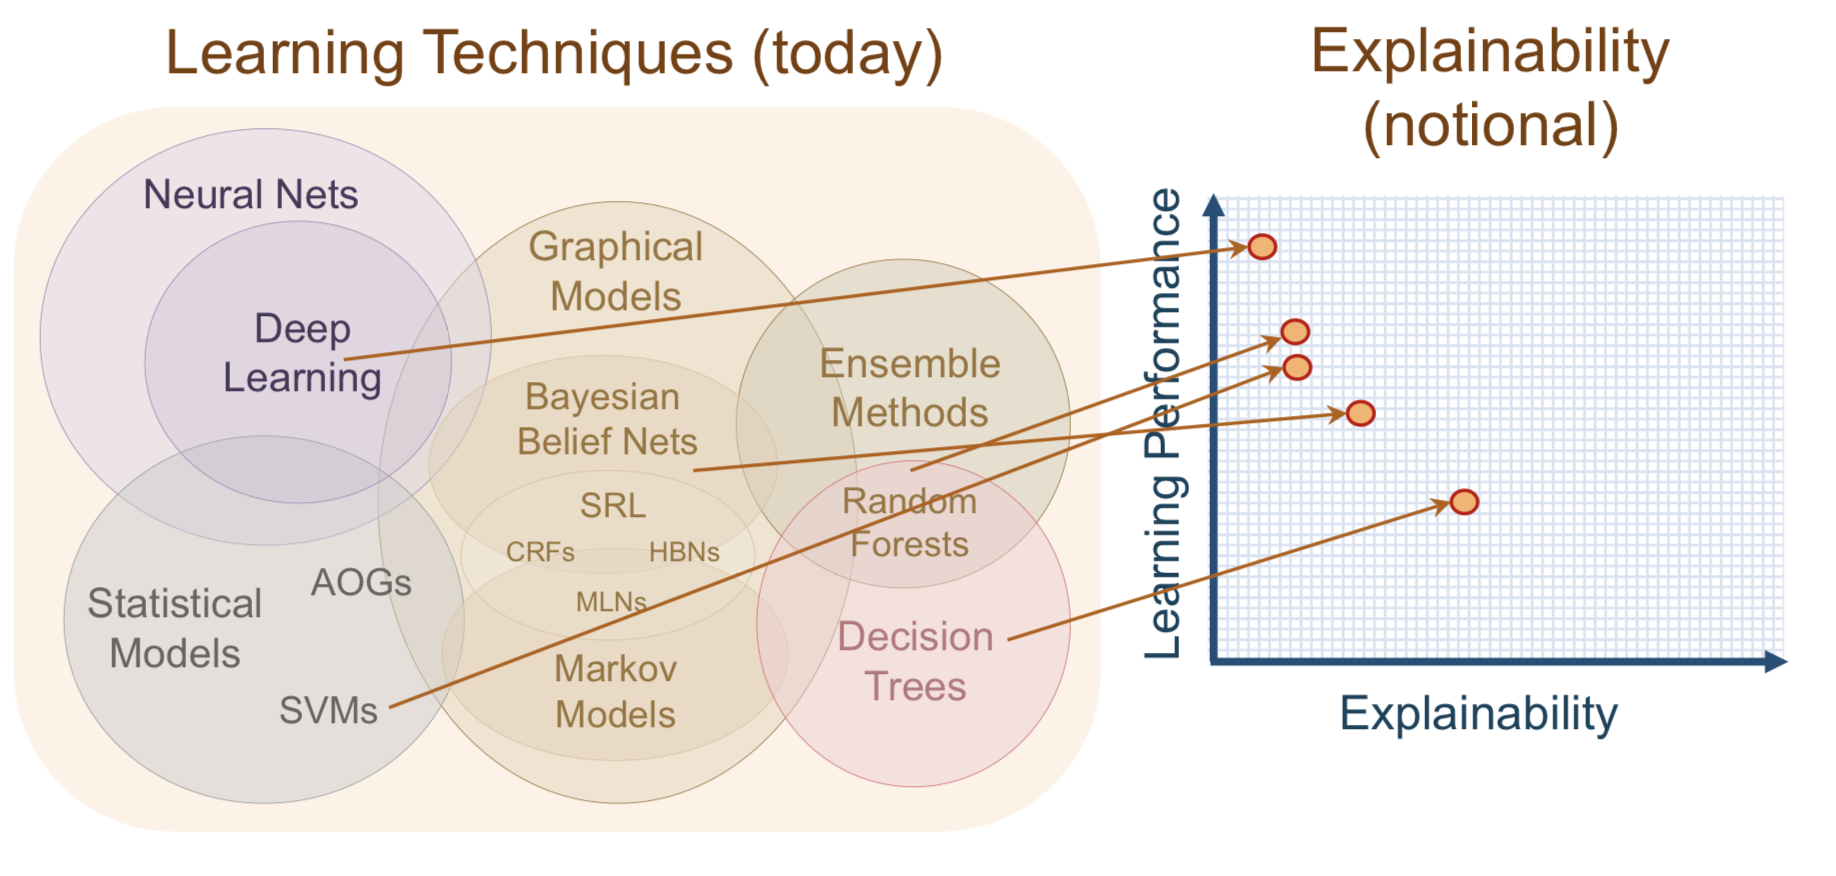
\includegraphics[width=\textwidth]{introduction/images/darpa-comparison-methods}}
\caption{Mapping showing the trade-off between performance and interpretability of contemporary and older machine learning models \citep{gunning2017explainable}.}
\label{fig:darpa-comparison-methods}
\end{figure}

The runaway success obtained by modern machine learning in a variety of domains, on a spectrum that goes from oceanography to social work, has created the desire to also apply these methods to mission-critical and traditionally more entrenched fields.  
A perfect example of an area exhibiting both these characteristics is that of medicine\footnote{For an overview of deep neural networks applied to medicine see \citet{Travers2018}.}.  
The first successful artificially intelligent systems date back to the 1970s and 1980s, these were based on \textit{symbolic methods} integrated with \textit{knowledge-bases}.  
These systems were, by design, capable of providing an explanation for their reasoning and were thus accepted by the medical community in an implementation known as \textit{expert systems}, which aimed to aid in the diagnosis of disease\footnote{For an overview of expert systems see \citet{Liao2005}.}. 
The insufficient ability of modern AI methods in being able to provide a justification for their reasoning has stunted their acceptance in the field of medicine, regardless of their superior performance and accuracy.

One modern ML model that has seen a modicum of success in the medical domain is that of \textit{Bayesian networks} (BNs) (defined in much greater detail in Section \ref{sec:bayesiannetworks}), a graphical and computationally efficient way of representing dependencies between variables of interest\footnote{For an overview of BNs in the medical domain see \citet{Lucas2001}.}.  
The graphical component is given by the fact that each variable is represented by a node of a directed acyclic graph (DAG) (Definition \ref{def:dag}), with the edges connecting them modelling their dependencies.  
The efficiency stems from the fact that the graph structure imposes a factorisation of the joint probability space and thus allows each variable's values be calculated using only those of its parents.
Bayesian networks may be uniquely suited to providing effective explanations by virtue of their inherent characteristics, as is discussed in detail in Section \ref{sec:explainability-in-bayesian-networks} below.

In a high-stakes domain such as the medical one, it would be unthinkable for a doctor to trust the predictions of an AI system \textit{a priori}.
Any decision with profound moral implications - such as prescribing or interrupting the treatment of a patient - would first have to be validated by a human; who would need to understand the rationale behind the machine's output to be able to do so. 
The feasibility of carrying out this validation is dependent on the degree of interpretability of the model that made the decision and, unfortunately, the lack of explainability methods tested in the real world are one of the main gaps identified in the field xAI.
BNs are no exception because, as noted by \citet{timmer2015explaining}, their underlying formalism makes them appear akin to \enquote{black-boxes} to domain experts, who are usually not well-versed in statistical reasoning.
Among other professionals, doctors certainly cannot be expected to double as machine learning experts. 
Therefore, the onus of developing comprehensible models falls squarely on the researchers in the xAI community.
Through a \textit{process of real-world validation and testing}, such researchers need to strive to develop methods that are not only provably correct but, just as importantly, confirmed in their capacity of relating efficiently to their users.

Explainability is necessary for a ML system's outputs to be verified and this, in turn, is a prerequisite for them to be applied in mission-critical domains.
Furthermore, explainability is also essential to be able to extract knowledge from data. 
The amount of information that a machine can process is many orders of magnitude greater than that inspectable by any human; this may allow for a computer to spot new patterns in the data, which would otherwise remain undetectable when observing only a limited amount of samples.   
The ability to understand the mapping from the model's inputs to its outputs can be seen as \textit{understanding the system's \enquote{reasoning} process} and could thus lead to new insights or to the confirmation of existing theories.
This is because understanding the process the model uses to give a certain output can make the machine's \textit{deep/vertical} analytical power available to our more \textit{general/horizontal} capacities.
This is also noted \textit{en passant} by \citet{doshi2017towards} when they state that \enquote{humans' goal is to gain knowledge. We do not have a complete way of stating what knowledge is; \textit{thus the best we can do is ask for explanations we can convert into knowledge}}.

Within this context, the main focus of this thesis is to address one of the most severe gaps in the current xAI literature: the lack of validation of machine learning systems with real expert users in concrete situations.
The work will focus in particular on the medical area and will attempt to assess the effectiveness of a Bayesian network-based system by means of an evaluation carried out in collaboration with expert clinicians in a real work setting, over a period of time.
The main hypothesis under investigation is if Bayesian networks may be inherently suited to being made explainable, compared to other ML models. 
Another objective is also to lay out the methodological groundwork for future research aimed at addressing the lack of \textit{human-centred evaluations}, that was found missing in the xAI literature.